
\FloatBarrier


\subsection{Logging Implementation}
\label{appendix:logging-implementation}

This section presents the descriptive results of the logging
implementation part of the developer survey. Eight respondents
completed the logging implementation questions ($n=8$). Two additional
survey participants did not implement logging and therefore did not
answer the remaining questions in this section. Unless stated
otherwise, all results in this subsection refer to these eight
respondents.



\begin{figure}[H]
    \centering
    \scriptsize


    \begin{minipage}[t]{0.48\textwidth}
        \centering

        \textbf{\scriptsize
        What percentage of your overall development time do you spend
        implementing logging?}

        \vspace{0.15em}

        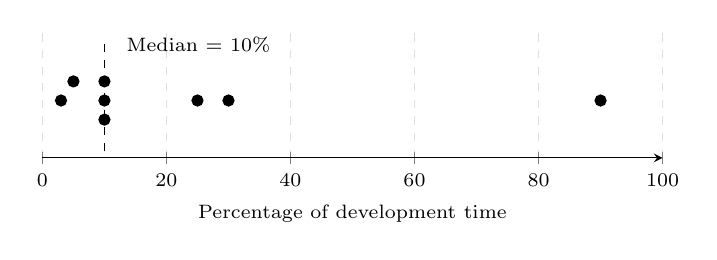
\begin{tikzpicture}
            \begin{axis}[
                width=0.78\linewidth,
                height=3.2cm,
                xmin=0,
                xmax=100,
                ymin=0.82,
                ymax=1.22,
                xtick={0,20,40,60,80,100},
                xlabel={Percentage of development time},
                xlabel style={font=\scriptsize},
                tick label style={font=\scriptsize},
                ytick=\empty,
                axis y line=none,
                axis x line=bottom,
                grid=major,
                grid style={dashed,gray!25},
                clip=false
            ]

            \addplot[
                only marks,
                mark=*,
                mark size=2pt
            ] coordinates {
                (3,1.00)
                (5,1.06)
                (10,0.94)
                (10,1.00)
                (10,1.06)
                (25,1.00)
                (30,1.00)
                (90,1.00)
            };

            \draw[dashed]
                (axis cs:10,0.84) --
                (axis cs:10,1.20);

            \node[
                anchor=south west,
                font=\scriptsize
            ] at (axis cs:12,1.12)
            {Median = 10\%};

            \end{axis}
        \end{tikzpicture}

        \par
        {\scriptsize
        (a) Development time spent implementing logging.}

    \end{minipage}\hfill%
    \begin{minipage}[t]{0.48\textwidth}
        \centering

        \textbf{\scriptsize
        What kind of data do you log?}

        \vspace{0.15em}

        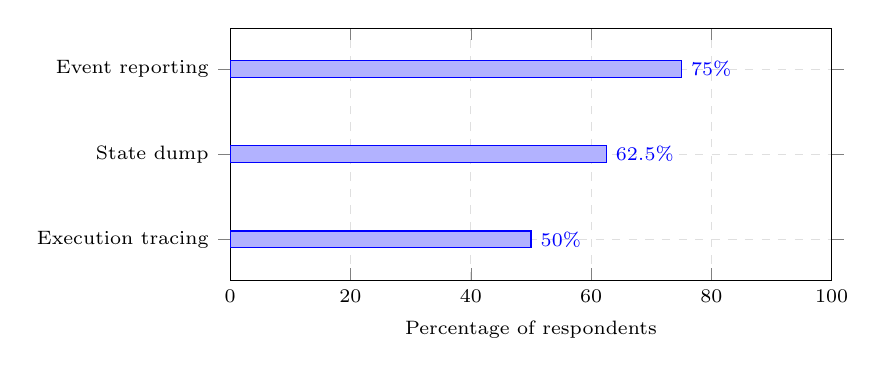
\begin{tikzpicture}
            \begin{axis}[
                xbar,
                width=0.63\linewidth,
                height=3.2cm,
                scale only axis,
                xmin=0,
                xmax=100,
                xtick={0,20,40,60,80,100},
                xlabel={Percentage of respondents},
                xlabel style={font=\scriptsize},
                symbolic y coords={
                    {Execution tracing},
                    {State dump},
                    {Event reporting}
                },
                ytick=data,
                yticklabel style={font=\scriptsize},
                tick label style={font=\scriptsize},
                nodes near coords={
                    \pgfmathprintnumber{\pgfplotspointmeta}\%
                },
                every node near coord/.append style={
                    font=\scriptsize
                },
                point meta=x,
                bar width=6pt,
                enlarge y limits=0.24,
                grid=major,
                grid style={dashed,gray!25}
            ]

            \addplot coordinates {
                (50,{Execution tracing})
                (62.5,{State dump})
                (75,{Event reporting})
            };

            \end{axis}
        \end{tikzpicture}

        \par
        {\scriptsize
        (b) Types of information logged according to the
        literature-derived \textit{What to log} categories.}

    \end{minipage}

    \par\vspace{0.35cm}

    \begin{minipage}[t]{0.48\textwidth}
        \centering

        \textbf{\scriptsize
        What methods or tools do you use for logging?}

        \vspace{0.15em}

        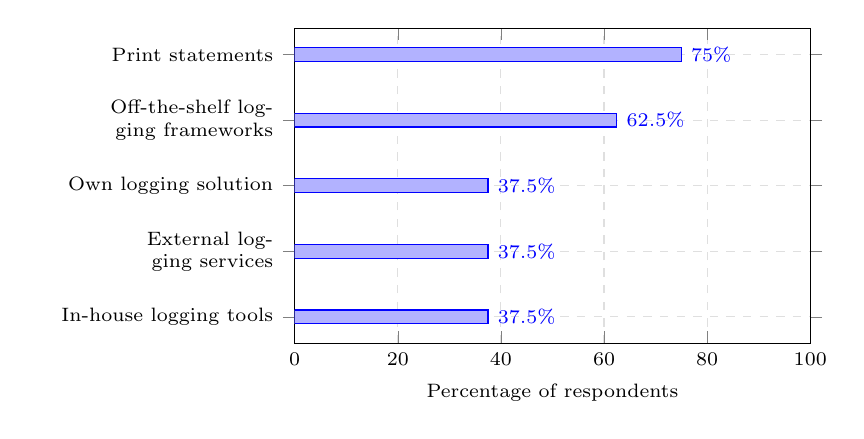
\begin{tikzpicture}
            \begin{axis}[
                xbar,
                width=0.54\linewidth,
                height=4.0cm,
                scale only axis,
                xmin=0,
                xmax=100,
                xtick={0,20,40,60,80,100},
                xlabel={Percentage of respondents},
                xlabel style={font=\scriptsize},
                symbolic y coords={
                    {In-house logging tools},
                    {External logging services},
                    {Own logging solution},
                    {Off-the-shelf logging frameworks},
                    {Print statements}
                },
                ytick=data,
                yticklabel style={
                    text width=3.0cm,
                    align=right,
                    font=\scriptsize
                },
                tick label style={font=\scriptsize},
                nodes near coords={
                    \pgfmathprintnumber{\pgfplotspointmeta}\%
                },
                every node near coord/.append style={
                    font=\scriptsize
                },
                point meta=x,
                bar width=5pt,
                enlarge y limits=0.10,
                grid=major,
                grid style={dashed,gray!25}
            ]

            \addplot coordinates {
                (37.5,{In-house logging tools})
                (37.5,{External logging services})
                (37.5,{Own logging solution})
                (62.5,{Off-the-shelf logging frameworks})
                (75,{Print statements})
            };

            \end{axis}
        \end{tikzpicture}

        \par
        {\scriptsize
        (c) Methods and tools used for logging.
        Multiple selections were possible.}

    \end{minipage}\hfill%
    \begin{minipage}[t]{0.48\textwidth}
        \centering

        \textbf{\scriptsize
        Which is the most common log format you use?}

        \vspace{0.15em}

        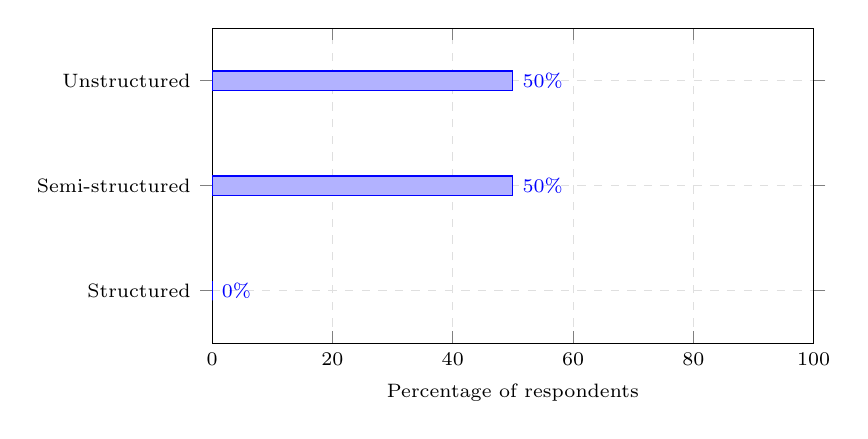
\begin{tikzpicture}
            \begin{axis}[
                xbar,
                width=0.63\linewidth,
                height=4.0cm,
                scale only axis,
                xmin=0,
                xmax=100,
                xtick={0,20,40,60,80,100},
                xlabel={Percentage of respondents},
                xlabel style={font=\scriptsize},
                symbolic y coords={
                    {Structured},
                    {Semi-structured},
                    {Unstructured}
                },
                ytick=data,
                yticklabel style={font=\scriptsize},
                tick label style={font=\scriptsize},
                nodes near coords={
                    \pgfmathprintnumber{\pgfplotspointmeta}\%
                },
                every node near coord/.append style={
                    font=\scriptsize
                },
                point meta=x,
                bar width=7pt,
                enlarge y limits=0.25,
                grid=major,
                grid style={dashed,gray!25}
            ]

            \addplot coordinates {
                (0,{Structured})
                (50,{Semi-structured})
                (50,{Unstructured})
            };

            \end{axis}
        \end{tikzpicture}

        \par
        {\scriptsize
        (d) Most commonly used log format.}

    \end{minipage}

    \caption{Selected descriptive results for logging implementation.
    Multiple selections were possible where applicable.}
    \label{fig:appendix-logging-overview}
\end{figure}



\clearpage

\begin{figure}[H]
    \centering

    \textbf{\scriptsize
    Based on which criteria do you determine how critical
    the information to log is?}

    \vspace{0.15em}

    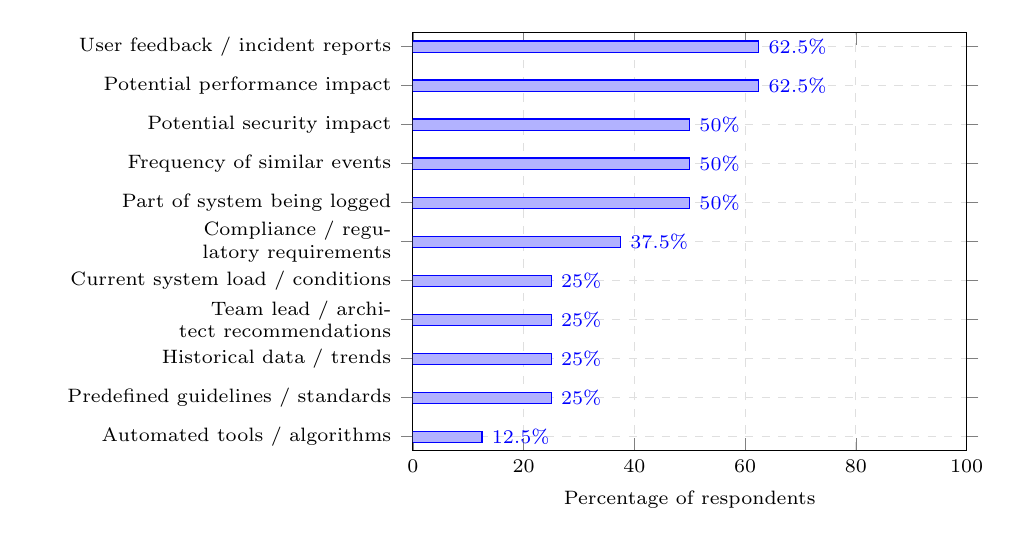
\begin{tikzpicture}
        \begin{axis}[
            xbar,
            width=0.58\textwidth,
            height=5.3cm,
            scale only axis,
            xmin=0,
            xmax=100,
            xtick={0,20,40,60,80,100},
            xlabel={Percentage of respondents},
            xlabel style={font=\scriptsize},
            symbolic y coords={
                {Automated tools / algorithms},
                {Predefined guidelines / standards},
                {Historical data / trends},
                {Team lead / architect recommendations},
                {Current system load / conditions},
                {Compliance / regulatory requirements},
                {Part of system being logged},
                {Frequency of similar events},
                {Potential security impact},
                {Potential performance impact},
                {User feedback / incident reports}
            },
            ytick=data,
            yticklabel style={
                text width=4.5cm,
                align=right,
                font=\scriptsize
            },
            tick label style={font=\scriptsize},
            nodes near coords={
                \pgfmathprintnumber{\pgfplotspointmeta}\%
            },
            every node near coord/.append style={
                font=\scriptsize
            },
            point meta=x,
            bar width=4pt,
            enlarge y limits=0.035,
            grid=major,
            grid style={dashed,gray!25}
        ]

        \addplot coordinates {
            (12.5,{Automated tools / algorithms})
            (25,{Predefined guidelines / standards})
            (25,{Historical data / trends})
            (25,{Team lead / architect recommendations})
            (25,{Current system load / conditions})
            (37.5,{Compliance / regulatory requirements})
            (50,{Part of system being logged})
            (50,{Frequency of similar events})
            (50,{Potential security impact})
            (62.5,{Potential performance impact})
            (62.5,{User feedback / incident reports})
        };

        \end{axis}
    \end{tikzpicture}

    \caption{Criteria used to determine the criticality of information
    to be logged. Multiple selections were possible.}
    \label{fig:appendix-criticality-criteria}
\end{figure}


\vspace{-0.4em}



\begin{figure}[H]
    \centering
    \scriptsize


    \begin{minipage}[t]{0.39\textwidth}
        \centering

        \textbf{\scriptsize
        How does the criticality of the information affect logging?}

        \vspace{0.15em}

        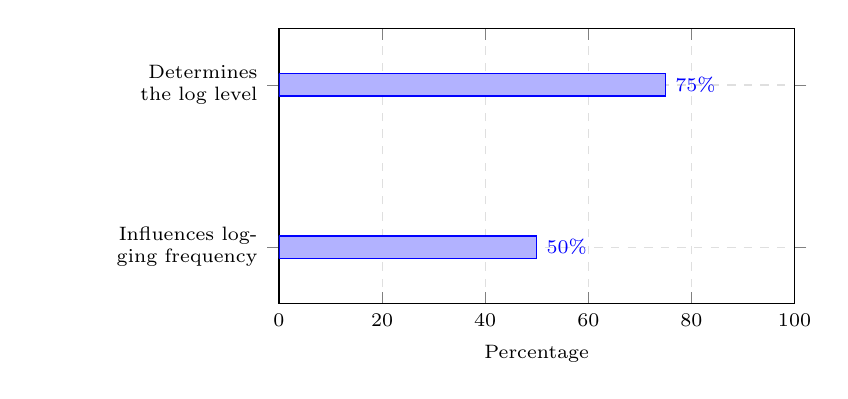
\begin{tikzpicture}
            \begin{axis}[
                xbar,
                width=0.54\linewidth,
                height=3.5cm,
                scale only axis,
                xmin=0,
                xmax=100,
                xtick={0,20,40,60,80,100},
                xlabel={Percentage},
                xlabel style={font=\scriptsize},
                symbolic y coords={
                    {Influences logging frequency},
                    {Determines the log level}
                },
                ytick=data,
                yticklabel style={
                    text width=2.8cm,
                    align=right,
                    font=\scriptsize
                },
                tick label style={font=\scriptsize},
                nodes near coords={
                    \pgfmathprintnumber{\pgfplotspointmeta}\%
                },
                every node near coord/.append style={
                    font=\scriptsize
                },
                point meta=x,
                bar width=8pt,
                enlarge y limits=0.35,
                grid=major,
                grid style={dashed,gray!25}
            ]

            \addplot coordinates {
                (50,{Influences logging frequency})
                (75,{Determines the log level})
            };

            \end{axis}
        \end{tikzpicture}

        \par
        {\scriptsize
        (a) Effect of information criticality.}

    \end{minipage}\hfill%
    \begin{minipage}[t]{0.59\textwidth}
        \centering

        \textbf{\scriptsize
        To which extent do you agree or disagree with the following
        statements?}

        \vspace{0.15em}

        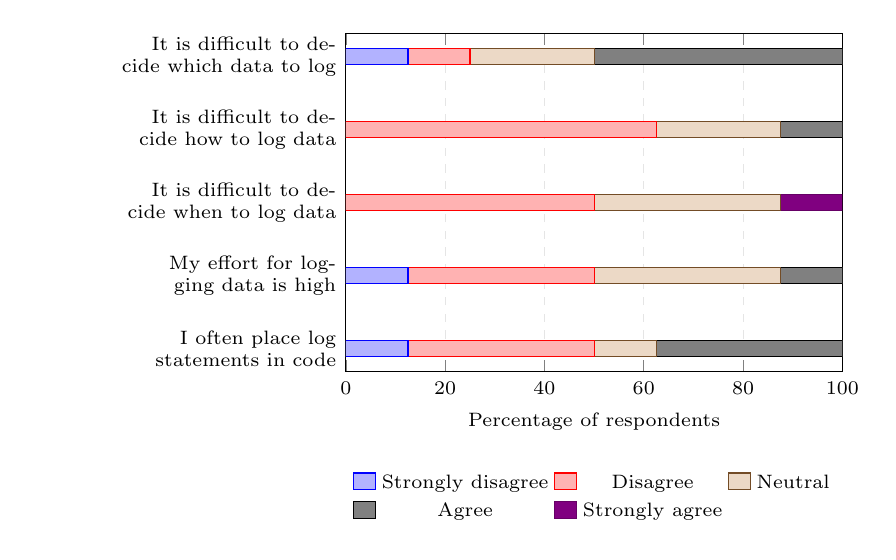
\begin{tikzpicture}
            \begin{axis}[
                xbar stacked,
                width=0.52\linewidth,
                height=4.3cm,
                scale only axis,
                xmin=0,
                xmax=100,
                xtick={0,20,40,60,80,100},
                xlabel={Percentage of respondents},
                xlabel style={font=\scriptsize},
                symbolic y coords={
                    {I often place log statements in code},
                    {My effort for logging data is high},
                    {It is difficult to decide when to log data},
                    {It is difficult to decide how to log data},
                    {It is difficult to decide which data to log}
                },
                ytick=data,
                yticklabel style={
                    text width=3.8cm,
                    align=right,
                    font=\scriptsize
                },
                tick label style={font=\scriptsize},
                bar width=6pt,
                enlarge y limits=0.08,
                legend style={
                    at={(0.5,-0.27)},
                    anchor=north,
                    legend columns=3,
                    font=\scriptsize,
                    draw=none
                },
                grid=major,
                grid style={dashed,gray!20}
            ]

            % Strongly disagree
            \addplot coordinates {
                (12.5,{I often place log statements in code})
                (12.5,{My effort for logging data is high})
                (0,{It is difficult to decide when to log data})
                (0,{It is difficult to decide how to log data})
                (12.5,{It is difficult to decide which data to log})
            };

            % Disagree
            \addplot coordinates {
                (37.5,{I often place log statements in code})
                (37.5,{My effort for logging data is high})
                (50,{It is difficult to decide when to log data})
                (62.5,{It is difficult to decide how to log data})
                (12.5,{It is difficult to decide which data to log})
            };

            % Neutral
            \addplot coordinates {
                (12.5,{I often place log statements in code})
                (37.5,{My effort for logging data is high})
                (37.5,{It is difficult to decide when to log data})
                (25,{It is difficult to decide how to log data})
                (25,{It is difficult to decide which data to log})
            };

            % Agree
            \addplot coordinates {
                (37.5,{I often place log statements in code})
                (12.5,{My effort for logging data is high})
                (0,{It is difficult to decide when to log data})
                (12.5,{It is difficult to decide how to log data})
                (50,{It is difficult to decide which data to log})
            };

            % Strongly agree
            \addplot coordinates {
                (0,{I often place log statements in code})
                (0,{My effort for logging data is high})
                (12.5,{It is difficult to decide when to log data})
                (0,{It is difficult to decide how to log data})
                (0,{It is difficult to decide which data to log})
            };

            \legend{
                Strongly disagree,
                Disagree,
                Neutral,
                Agree,
                Strongly agree
            }

            \end{axis}
        \end{tikzpicture}

        \par
        {\scriptsize
        (b) Perceptions of logging implementation.}

    \end{minipage}

    \caption{Effects of criticality and respondents' perceptions of
    logging implementation.}
    \label{fig:appendix-criticality-and-perceptions}
\end{figure}


\clearpage

\subsubsection{Open-Ended Logging Implementation Responses}
\label{appendix:open-ended-logging-implementation}

The following table presents lightly paraphrased versions of the
open-ended survey responses. Responses were rephrased for readability
and conciseness while preserving their original meaning. No additional
thematic coding was applied.

\vspace{0.3em}

\begin{table}[H]
    \centering
    \scriptsize

    \caption{Paraphrased open-ended responses concerning logging
    implementation.}
    \label{tab:appendix-logging-open-responses}

    \begin{tabularx}{\textwidth}{
        @{}
        >{\centering\arraybackslash}p{0.035\textwidth}
        >{\RaggedRight\arraybackslash}p{0.29\textwidth}
        >{\RaggedRight\arraybackslash}p{0.31\textwidth}
        >{\RaggedRight\arraybackslash}X
        @{}
    }

        \toprule

        \textbf{ID} &
        \textbf{Colleague involvement} &
        \textbf{Challenges} &
        \textbf{Effective strategies} \\

        \midrule

        P1 &
        The response focused on tracing errors back to the specific
        method or class rather than direct colleague involvement. &
        Outside classes with established logging, it can be unclear
        where and what to log. &
        Use a clear, readable, and well-structured log file. \\

        \addlinespace[0.2em]

        P2 &
        Colleagues are not involved. &
        No specific difficulties were reported. &
        No particular strategy was reported. \\

        \addlinespace[0.2em]

        P3 &
        Colleagues are not involved, mainly because the respondent has
        not worked on larger collaborative projects. &
        Performance-related logging statements can be difficult to place;
        therefore, a larger amount of information may be logged. &
        Use third-party applications for error logging. \\

        \addlinespace[0.2em]

        P4 &
        The response focused on using logs to identify errors rather than
        direct colleague involvement. &
        The purpose and subsequent use of collected logging metrics can
        be unclear. &
        Add logs at module or component level to trace execution flow. \\

        \addlinespace[0.2em]

        P5 &
        Colleagues are not involved. &
        No specific difficulties were reported. &
        No relevant experience with logging strategies was reported. \\

        \addlinespace[0.2em]

        P6 &
        Colleagues may be consulted about relevant data and logging
        requirements affecting architecture or component design. &
        Logging itself is usually not difficult, but suitable logging
        options should be considered during architecture and design. &
        Use the same framework where possible and avoid both excessive
        and insufficient logging. \\

        \addlinespace[0.2em]

        P7 &
        Colleagues are not directly involved, but logs are written so
        they can analyse them later. &
        Finding a concise and readable log format can be challenging. &
        Log incoming and outgoing data. \\

        \addlinespace[0.2em]

        P8 &
        The team discusses and defines how logging should be implemented. &
        Designing how data should be displayed in a custom log format
        can be difficult. &
        Write meaningful entries, sample logs, and consider logging
        performance costs. \\

        \bottomrule

    \end{tabularx}
\end{table}



\FloatBarrier
\clearpage